\chapter{Onderzoeksplan}\label{ch:onderzoekPlan}

In het vorige hoofdstuk is de opdracht voor dit onderzoek beschreven. In dit hoofdstuk wordt uitgewijd over hoe deze opdracht en het daarbij behorende onderzoek zal worden uitgevoerd en welke bronnen er hiervoor gebruikt worden. Het resultaat is een onderzoeksplan voor een onderzoek naar analyses op kwetsbaarheden in externe bibliotheken (SOUP) binnen Eaglescience.


\section{Aanleiding}\label{sec:OP_aanleiding}
Eaglescience heeft de ambitie om te groeien in zowel het aantal projecten dat het aanneemt als in het aantal medewerkers. Daarnaast is het bezig met het integreren van het software lifecycle management paradigma in het kwaliteitssysteem om zo een gerichte-, transparante en traceerbare aanpak te hebben aangaande de kwaliteit en daarmee de veiligheid van de te leveren software. Er wordt gezocht naar manieren om taken die veel voorkomen en bijdragen aan de kwaliteit te automatiseren om op die manier een traceerbare en transparante aanpak te verkrijgen. Op dit moment mist voornamelijk inzicht in de kwetsbaarheden van projecten waarvan de ontwikkeling is afgerond, maar die wel door Eaglescience worden gehost en daardoor onder haar verantwoordelijkheid vallen.


\section{Probleemanalyse}\label{sec:probleemanalyse}
Eaglescience doet veel om veilige applicaties te leveren aan haar klanten. Tijdens het ontwikkelproces wordt er door de ontwikkelaars continue afgewogen welke maatregelen, in architectuur en/of code, moeten worden genomen om applicaties veilig op te kunnen leveren. Deze afwegingen zijn onderdeel van het ontwerpproces en worden door de klant gezien als declarabele uren en zij zijn dan ook bereid voor deze werkzaamheden te betalen. Op het moment dat een project "klaar" is en over gaat van ontwikkeling naar hosting wordt er onderhoud gedaan volgens afspraken in de SLA. In diezelfde SLA wordt niet altijd ruimte opgenomen voor het testen van de applicatie op kwetsbaarheden middels SOUP-analyses. Vaak komt dit doordat de klant er geen budget voor heeft, of het niet belangrijk vindt. Gezien Eaglescience alleen een advies kan uitbrengen over support en de klant de eindbeslissing neemt worden SOUP-analyses veelal niet of niet tijdig uitgevoerd. Omdat Eaglescience wel "zo veel mogelijk" wil garanderen dat de software die gehost wordt veilig is, dient de applicatie in hosting periodiek geannalyseerd te worden op kwetsbaarheden. Op dit moment is dit een tijdrovend handmatig process waarmee een teamlid ongeveer 8 tot 12 uur bezig is. Voor iedere dependency moet er namelijk bekeken worden of er mogelijke kwetsbaarheden bestaan, of dan al niet upgedate moeten worden. Door de groei die Eaglescience binnekort wil maken bestaat de wens om bovenstaand proces te automatiseren.

Er moet dus een methode worden ontwikkeld die het mogelijk maakt om geautomatiseerd en periodiek een SOUP-analyse te doen op dependencies binnen een project. De SOUP-analyses moeten inzichtelijk maken of en zo ja, welke, kwetsbaarheden zijn gevonden in deze bibliotheken. De methode moet voor alle platformen (Docker, programmeertalen, databases etc.) dezelfde resultaten geven, en compatible zijn met de huidige infrastructuur van Eaglescience.

Door de analyses te automatiseren wordt beoogd dat er minder tijd zal hoeven worden besteed aan de analyse. Deze tijd kan dan worden ingezet door de ontwikkelaar aan taken die declarabel zijn en voor beide partijen winstgevend zijn.


\section{Probleem stelling, onderzoeksvraag en doelstellingen}\label{sec:probleem-stelling-onderzoeksvraag-en-doelstellingen}
Samengevat luidt het probleem: "Het handmatig uitvoeren van SOUP-analyses kost manuren die niet declarabel zijn. Om deze reden is de wens dat er een geautomatiseerde oplossing komt die periodiek de projecten, die in ontwikkeling zijn en/of door Eaglescience gehost worden, analyseerd op kwetsbaarheden in gebruikte externe bibliotheken. Door deze automatische oplossing te gebruiken wordt beoogd dat de (niet declarabele) uren die normaal gebruikt worden voor het analyseren van projecten in plaats daarvan gebruikt kunnen worden voor andere wel declarabale uren. Hierdoor zou de efficientie binnen Eaglescience kunnen worden verhoogd.

Voor het onderzoek naar het hierboven genoemde probleem is de volgende centrale onderzoeksvraag opgesteld: "Hoe kan Eaglescience middels een geautomatiseerde methode inzicht krijgen in potentiële kwetsbaarheden van gebruikte bibliotheken binnen projecten, waarbij rekening gehouden wordt met de huidige manier van werken?"

De opdracht heeft de volgende doelstelling:
Het doel van dit onderzoek is het ontwikkelen van een methode om SOUP-analyses uit te voeren binnen de dev-stack van Eaglescience. Hierbij moet rekening gehouden worden met de in de opdracht gegeven criteria. Aan het einde van het onderzoek moet een methode worden gepresenteerd die vervolgens bewezen kan worden middels een implementantie van een analyse op de twee meest gebruikte technologiën binnen Eaglescience.


\section{Stakeholdersanalyse}\label{sec:stakeholdersanalyse}
Om inzicht te verkrijgen in het draagvlak voor dit onderzoek dient er een stakeholders analyse gedaan te worden. Op deze manier moet het duidelijk worden wie de stakeholders zijn en welke belangen zij hebben bij het doen van een onderzoek naar een geautomatiseerde SOUP-analyse en de resultaten hiervan.

\subsection{Dagelijks bestuur (intern)}\label{subsec:dagelijks-bestuur-(intern)1}
Het dagelijks bestuur ziet vooral voordelen in het op een overzichtelijke manier verkrijgen van inzichten in kwetsbaarheden. Zij beogen dat ze hierdoor beter kunnen aansturen in het gebruik van bibliotheken en/of andere technologiëen. Ondanks dat de ontwikkeling van de beoogde nieuwe module vooral geld zal kosten, is de huidige manier van werken ook niet kosten-effectief. Daarnaast voorziet de CTO dat de nieuwe module tijdswinst zal opleveren waardoor de time-to-market voor andere projecten hoger kan komen te liggen en er dus op langer termijn meer omzet gegenereerd kan worden.

\subsection{Projectmanagers (intern)}\label{subsec:projectmanagers-(intern)1}
Project managers krijgen op dit moment een update over de staat van kwetsbaarheden na afronding van een analyse, welke veelal na een deploy plaatsvindt of op verzoek. De nieuwe module zal echter de mogelijkheid bieden om up-to-date informatie on-demand te verkrijgen.
De tijdsinvestering die nodig is van ontwikkelaars voor de ontwikkeling van de module weegt volgens hen op tegen de voordelen die de module in de toekomst kan brengen.

\subsection{Ontwikkelteam (intern)}\label{subsec:ontwikkelteam-(intern)1}
Het handmatig testen van kwetsbaarheden werd tot op heden gedaan door het ontwikkelteam. Dit is een tijdrovende taak, welke ten koste gaat van de ontwikkeling van software voor klanten. Het ontwikkelteam heeft daarom direct baat bij de ontwikkeling van de beoogte module en wil daarom graag hieraan meedenken en meewerken.

\subsection{Klant (extern)}\label{subsec:klant-(extern)1}
De enige externe stakeholder is de klant. Dit is tevens een passieve stakeholder gezien zij niet direct betrokken zijn bij de ontwikkeling van de module, maar wel baat hebben bij de uitkomst hiervan, namelijk in de vorm van veiligere en betrouwbaardere software tegen potentieel lagere kosten.

\begin{figure}[H]
    \myfloatalign
    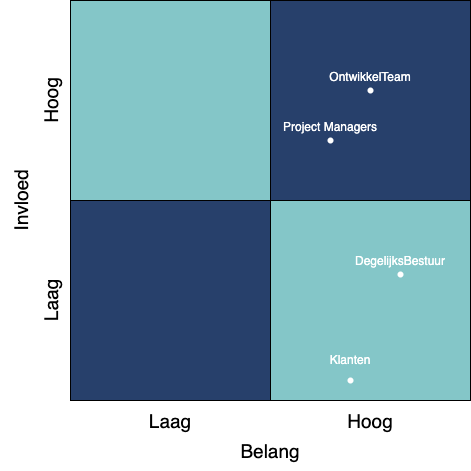
\includegraphics[width=10cm]{gfx/stakeholderanalyse}
    \caption{StakeHolders Analyse}
    \label{fig:StakeholderAnalyse1}
\end{figure}
Zoals te zien is in figuur~\ref{fig:StakeholderAnalyse1} is hebben alle stakeholders veel baat bij een nieuwe module voor de analyse van kwetsbaarheden. De invloed hierop is het hoogst bij het ontwikkelteam en de projectmangagers. De lage invloed van de klant zorgt ervoor dat voor het ontwerp alleen de requirements vanuit Eaglescience worden opgenomen.

\section{Theoretisch kader}\label{sec:theoretisch-kader}
Het theoretisch kader waarmee wordt gewerkt bestaat uit twee delen. Het eerste deel omvat theorie over externe bibliotheken. Het richt zich op het gebruik hiervan en de potentiële gevaren en methoden om deze bibliotheken te analyseren. De geselecteerde bronnen zijn:
\begin{itemize}
    \item \textbf{OWASP top 10 (https://owasp.org/Top10/)} De OWASP Top-10 is als uitgangspunt gekozen omdat de inhoud van dit document binnen Eaglescience geldt als aandachtspunt voor het ontwikkelen van veilige software. De basis voor dit onderzoek wordt beschreven in punt "A06:2021-Vulnerable and Outdated Components". Hier wordt beschreven welke gevaren er potentieel dreigen als op dit punt niets gedaan wordt.
    \item \textbf{Detail pagina OWASP A06:2021\\(https://owasp.org/Top10/A06\_2021-Vulnerable\_and\_Outdated\_Components/)} Op deze pagina zijn details te vinden over item A06:2021 waaronder een beschrijving, hoe het te voorkomen is en een aantal voorbeeld scenario's waarbij een aanval wordt geillustreerd.
    \item \textbf{OWASP dependency-check (https://owasp.org/www-project-dependency-check/)} Pagina over het project binnen de OWASP voor het analyseren van componenten in applicaties.
    \item \textbf{Justifying the use of software of uncertain pedigree (SOUP) in safety-related applications} P.G.\ Bishop, R.E.\ Bloomfield and P.K.D.\  Froome for Adelard 2001. Hoewel dit document verouderd lijkt staat er wel degelijk interessante informatie over waarom je SOUP zou gebruiken en hoe je de risico's kan verminderen.
    \item \textbf{Backstabber’s Knife Collection: A Review of Open Source Software Supply Chain Attacks} Marc Ohm, Henrik Plate, Arnold Sykosch, and Michael Meier: 2020: Dit artikel bevat informatie over een mogelijke vorm van aanvallen die middels SOUP uitgevoerd zouden kunnen worden. Daarnaast geeft het artikel inzicht in hoe de onderzoekers packages voor NPM, Python, en Ruby hebben onderzocht op kwetsbaarheden.
\end{itemize}
Het tweede deel omvat de werkwijze van Eaglescience en de door hun gebruikte technologiëen. De geselecteerde documenten vormen de basis informatie over de werkwijze van Eaglescience en zal als input worden gebruikt bij het ontwerp van de analyse welke aansluitend aan het onderzoek zal plaatsvinden. De volgende bronnen zullen bij het onderzoek worden gebruikt:
\begin{itemize}
    \item \textbf{151030 F04B Proces Flow Chart ES\_V1.0\_TN.pdf} Een document dat de workflow beschrijft die binnen Eaglescience gehanteerd wordt.
    \item \textbf{200121\_Policy Manual\_ES\_V6 signed.pdf} ISO handboek waarin de bedrijfsvoering binnen Eaglescience wordt beschreven.
\end{itemize}

\section{Conceptueel model}\label{sec:conceptueel-model}
Om de relevantie en relatie van de verschillende onderzoeken te waarborgen is het volgende conceptueel model opgesteld.
\begin{figure}[H]
    \centering
    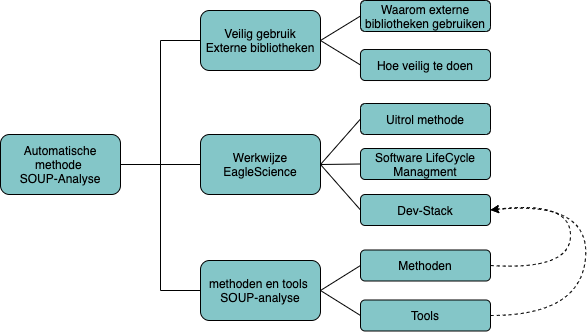
\includegraphics[width=12cm]{gfx/Conceptueel Model}
    \caption{Conceptueel Model}
    \label{fig:ConceptueelModel}
\end{figure}

In figuur~\ref{fig:ConceptueelModel} is het conceptueel model opgenomen dat voor deze opdracht is opgesteld. Dit model maakt de samenhang van de verschillende begrippen inzichtelijk.

Het kernbegrip is "Automatische methode SOUP-analyse" welke dit onderzoek uiteindelijk moet opleveren. Om hiertoe te komen zijn er drie begrippen die ieders een eigen domein binnen de probleemstelling belichten. In het theoretisch deel "Veilig gebruik externe bibliotheken" wordt onderzocht waarom er bibliotheken van buitenaf worden gebruikt en wat de potentiële gevaren zijn die dit met zich meebrengt, en eventuele remedies hiervoor. Daarna zal "Werkwijze Eaglescience" de manier van werken binnen Eaglescience belichten als ook de manier van uitrollen en de algehele dev-stack die Eaglescience gebruikt. Ook komt hier de Software Lifecycle Managment aan bod gezien dit één van de aanleidingen is van deze opdracht. Het begrip "Methoden en tools SOUP-analyse" zal ingaan op de beschikbare tools die gebruikt kunnen worden om een analyse te doen. Met deze tools wordt een methode onderzocht die SOUP-analyses mogelijk maakt binnen de dev-stack van Eaglescience. Tesamen zal dit onderzoek resulteren in een theoretische methode die als input kan gelden voor het ontwerp voor de nieuwe module die in de opdracht staat beschreven.


\section{Onderzoeksontwerp}\label{sec:OP_onderzoeksontwerp}
Aan de hand van de hierboven beschreven doelstellingen, theoretisch kader en conceptueel model is het volgende onderzoeksontwerp opgesteld.

\subsection{Onderzoeksvraag}\label{subsec:onderzoeksvraag-en-deelvragen}
Op basis van de probeemanalyse luidt de onderzoeksvraag als volgt: "Hoe kan Eaglescience middels een geautomatiseerde methode inzicht krijgen in potentiële kwetsbaarheden van gebruikte bibliotheken binnen projecten waarbij rekening gehouden wordt met de huidige manier van werken?"

Door het ontleden van deze onderzoeksvraag onstaan er twee delen waarnaar onderzoek gedaan moet worden. Het eerste deel is het gebruik en gevaar van externe bibliotheken, welke leidt tot de volgende onderzoeksvraag: "Wat is het effect van het gebruik van externe bibliotheken bij het ontwikkelen van software, welke gevaren brengt dit met zich mee en wat kan er gedaan worden om deze gevaren te minimaliseren?". Vervolgens kan deze kennis worden benut in het tweede deel, wat de praktische kant belicht gericht op de methode en tooling voor SOUP-analyses. Dit tweede deel omvat methodes om geautomatiseerd SOUP-analyses te doen op projecten binnen Eaglescience. De onderzoeksvraag luidt als volgt: "Welke SCA tooling is compabitble met de omgeving van Eaglescience en welke methode kan worden toegepast om deze tooling te gebuiken voor het automatisch analyseren van externe dependencies?"

Deze delen zullen ieders in een deelonderzoek worden behandeld, waarvan de uitkomsten elkaar zullen aanvullen en samen tot een eind eindresultaat leiden.
\begin{figure}[H]
    \myfloatalign
    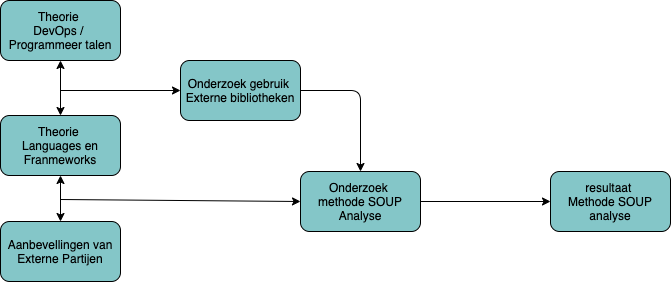
\includegraphics[width=10cm]{gfx/Onderzoekmodel}
    \caption{Onderzoeksmodel}
    \label{fig:OnderzoeksModel}
\end{figure}

In figuur\ref{fig:OnderzoeksModel} is te zien hoe de twee delen met elkaar in relatie staan ten opzichte van het beoogde eindresulaat. Het onderzoek over het gebruik van externe bibliotheken zal leiden tot concrete inzichten die vervolgens gebruikt kunnen worden als kennis in het onderzoek naar een methode voor een SOUP-analyse. Dit zal uiteindelijk een methode opleveren die gebruikt kan worden voor de implementatie van de module die aan de opdracht voldoet.

\subsection{Scope}\label{subsec:scope}
Het domein softwareveiligheid is op het moment van schrijven een 'hot-topic', en zeer breed. Om deze reden is er gekozen om dit onderzoek te beperken tot het veiliger maken van software middels het analyseren en beschikbaar stellen van informatie over externe bibliotheken. Daarnaast zullen alleen de technologiën die compatibel zijn met de werkwijze van Eaglescience mee worden genomen. Daarnaast is de opdracht\ref{ch:opdracht} zoals deze is gegeven door de CTO van Eaglescience de leidraad voor de scope van het onderzoek.

\subsection{Onderzoeks strategie}\label{subsec:onderzoeks-strategie}
Zoals hierboven is aangegeven zullen er een tweetal onderzoeken worden uitgevoerd. De conclusie van het eerste onderzoek zal dienen als input voor het tweede onderzoek.

%\newpage %TODO: quickfix om volgorde lijkheid te veranderen voor figuren...


\subsubsection{Onderzoek 1: gebruik externe bibliotheken, het gevaar en hoe veiliger te maken}
Het \textbf{doel} van dit onderzoek is om inzicht te krijgen wat een SOUP-analyse is en hoe relevant het is om deze uit te voeren. Daarnaast wordt er gekeken wat de SOUP-analyse toevoegd aan de veiligheid van de software die Eaglescience levert en hoe Eaglescience mogelijk kan voorkomen dat er kwetsbaarheden in de uitgerolde software terecht komt.
De \textbf{scope} van dit onderzoek is dat er gekeken wordt naar het gebruik van externe bibliotheken en de toegevoegde waarde hiervan. Daarnaast wordt er gekeken wat er gedaan kan worden om het gebruik van externe bibliotheken veiliger te maken.
De \textbf{onderzoeksvraag} luid: "Wat is het effect van het gebruik van externe bibliotheken bij het ontwikkelen van software, welke gevaren brengt dit met zich mee en wat kan er gedaan worden om deze gevaren te minimaliseren?".
De gebruikte \textbf{methodes} zullen deskresearch zijn aangevuld met conferenties, waarbij \textbf{bronnen} zoals artikelen en rapportages van instanties en bedrijven die zich bezighouden met de veiligheid van software zullen worden opgenomen met als focus het gebruik van externe bibliotheken. Software veiligheid is een 'hot-topic' en er worden jaarlijks veel conferenties gehouden over dit onderwerp. Door de huidige wereld situatie is het mogelijk om veel van deze conferenties "on-demand" terug te kijken wat op zijn beurt ook weer tot andere inzichten kan leiden. In figuur~\ref{fig:OnderzoeksModelNoodZaakSOUP} is te zien hoe het onderzoek is opgebouwd.
\begin{figure}[htbp]
    \myfloatalign
    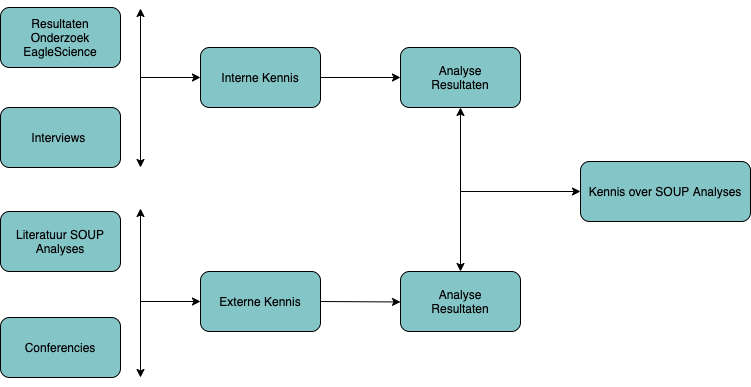
\includegraphics[width=10cm]{gfx/OnderzoeksmodelSOUP}
    \caption{Onderzoeks model gevaren van SOUP}
    \label{fig:OnderzoeksModelNoodZaakSOUP}
\end{figure}



\subsubsection{Onderzoek 2: tools en methodes voor SOUP-analyses op de Eaglescience dev-stack}\\
Het \textBF{doel} van dit onderzoek is om een methode te vinden die het mogelijk maakt om een SOUP-analyse te doen binnen de huidige dev-stack van Eaglescience. Hiervoor zullen er geschikte SCA (Software Composition Analysis) tools gevonden moeten worden.
Binnen de \textbf{Scope} van het onderzoek zal daarom alleen gekeken worden naar SCA tooling die analyses doet voor componenten binnen de dev-stack van Eaglescience.
De \textbf{Onderzoeksvraag} luidt: "Welke SCA tooling is compabitble met de omgeving van Eaglescience en welke methode kan worden toegepast om deze tooling te gebuiken voor het automatisch analyseren van externe dependencies?"
De \textbf{methode} die gebruikt wordt is deskresearch. Daarnaast zullen er interviews gehouden worden met collega's om inzicht te krijgen in de huidige stand van zaken op het gebied van gebruik van externe bibliotheken en hoe er in de huidige situatie voor wordt gezorgd dat er geen kwetsbaarheden worden geintroduceerd door het gebruik hiervan.

Als er een selectie is gemaakt voor een tool dient deze in een kleine testopstelling getest te worden om vervolgens te kijken of deze kan worden geimplementeerd in de bestaande uitrolmethode. De \textbf{bronnen} die gebruikt zullen worden zijn informatie bronnen van leveranciers van dergelijke tooling. Ook zal er in interne documentatie worden gekeken hoe de huidige processen draaien waarin wordt beoogd om de SOUP-analyse uit te voeren. Daarnaast zullen de bevindingen middels een review worden geverifieerd op bruikbaarheid bij de opdrachtgever. Het onderzoeksmodel voor dit onderzoek is te vinden in figuur~\ref{fig:OnderzoeksModelSOUPmethode}

\begin{figure}[htbp]
    \myfloatalign
    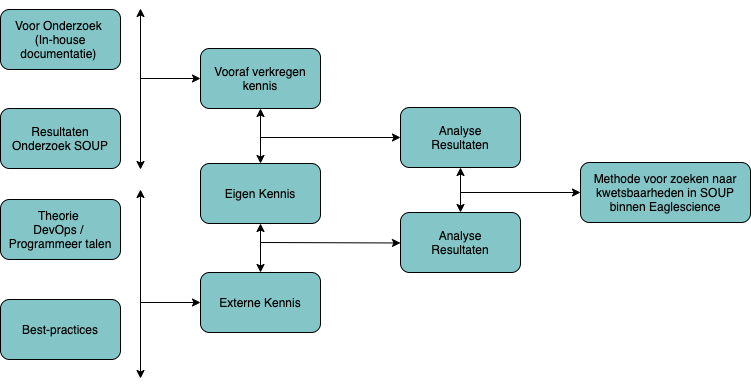
\includegraphics[width=10cm]{gfx/OnderzoeksModelSOUPMethode}
    \caption{Onderzoeksmodel SOUP-analyse module}
    \label{fig:OnderzoeksModelSOUPmethode}
\end{figure}

\section{planning}\label{sec:planning}
Om tijdig tot resultaten te komen is de volgende planning opgesteld.

\subsection{Requirements analyse \textbf{september 2021}}\label{subsec:requirements-analyse}
Na het ontvangen van de opdracht dient er onderzocht te worden of er naast de eisen die door de CTO in de opdracht zijn gezet nog andere eisen zijn binnen Eaglescience. Hiervoor zal er onderzocht worden welke betrokkenen er zijn en welke belangen en wensen zij hebben. Na het houden van interviews zullen alle wensen tegen elkaar worden afgewogen. Dit zal leiden tot een document waarin alle belangrijke requirements worden geprioriteerd volgens de MoSCoW\-methode.

\textbf{Methode:} Intake gesprek met opdrachtgever, interviews met betrokkenen, enquete voor ontwikkelaars.

\textbf{Resultaat:} Applicatie requirements document.

\subsection{Vooronderzoek \textbf{september 2021 - oktober 2021 }}\label{subsec:onderzoek}
Om de requirements om te kunnen zetten naar een ontwerp zal er onderzoek gedaan worden naar de huidige manier van ontwikkelen en compileren van de software. Een onderzoek naar begrippen binnen het domein SOUP is een voorwaarde om vervolgens onderzoek te kunnen doen naar methodes om analyses te kunnen doen op software die Eaglescience maakt ten opzichte van SOUP. De resultaten van het vooronderzoek zullen worden gebruikt als input.
Om meer kennis en verdieping te krijgen in de materie rondom de nieuwe module zullen er een aantal onderzoeken worden uitgevoerd.


Er is onderzoek nodig naar de volgende onderwerpen:
\begin{itemize}
    \item \textbf{Externe bibliotheken gebruik en het gevaar} Onderzoek naar waarom er externe bibliotheken worden gebruikt en het gevaar hiervan. En hoe deze kunnen worden ondervangen.
    \item \textbf{Soup Analyse binnen Eaglescience}Dit onderzoek zal de tooling en methode in kaart brengen voor het uitvoeren van SOUP-analyses binnen Eaglescience.
\end{itemize}

\textbf{Methode:} Bureau onderzoek, interviews met specialisten, deelnemen aan en/of terugkijken van conferenties, Sandbox testen met gevonden tooling

\textbf{Resultaat:} Inzicht in het begrip SOUP en software veiligheid als ook een idee voor een mogelijke implementatie van de oplossing die voor Eaglescience de beste is zonder veel impact op de huidige manier van werken te hebben.

\subsection{Initieel ontwerp \textbf{oktober 2021 - november 2021 }}\label{subsec:initieel-ontwerp}
Er zal een ontwerp worden gemaakt waarin vast gelegd is welke requirements er beslist in de module moeten zitten en de uitwerking van deze. Evenals een ontwerp van de architectuur en het datamodel. Naast de module zal er ook een ontwerp gemaakt worden voor een ontwikkel/test omgeving om de module continue te kunnen testen zonder dat dit de huidige buildstraat beinvloed. Dit laatste is van belang om zo min mogelijk storingen te veroorzaken in de dagelijkse gang van zaken bij al lopende projecten. Het eerste ontwerp zal als leidraad dienen voor de implementatie waarin afgeweken kan worden als dit nodig blijkt tijdens de implementatie sprints.

\textbf{Methode:} Overleggen met ontwikkelaars, huidige omgeving onderzoeken op mogelijkheden en architectuur.
\textit{wellicht nog toevoegen als resultaten: blokdiagram van oplossing/architectuur; sequence diagram om te komen van analyse tot rapportage (er is een handig tooltje om deze diagrammen te tekenen: https://bramp.github.io/js-sequence-diagrams/)}
\textbf{Resultaat:} Eerste ontwerp in de vorm van een datamodel, blokdiagram van architectuur voor de oplossing, als ook een sequence diagram om van analyse tot rapportage te komen.

%\textit{4.4: Gebruik hier of de template ontwikkel omgeving voor (aparte branch/taak); of de portal ontwikkelomgeving
%4.4: Voeg rij resultaat toe: klaar voor review of gereviewde}

\subsection{Implementatie en Testen \textbf{november 2021 - januari 2022 }}\label{subsec:implementatie-en-testen}
Om te kunnen beginnen aan de implementatie is er een ontwikkel/ test omgeving nodig die het mogelijk maakt om zonder invloed op de dagelijkse werkzaamheden van Eaglescience een module te kunnen ontwikkelen. Deze zal eerst worden opgezet. Als test projecten zullen snapshots worden gebruikt van de daadwerkelijke projecten dit om een zo accuraat mogelijke test omgeving te hebben. Zoals in de opdracht beschreven dient de nieuwe module een onderdeel te zijn van de bestaande portal. Er zal dan ook direct samen worden gewerkt met het team die daar op het moment mee aan het ontwikkelen is. Tijdens de implementatie zal er ook worden gedocumenteerd wordt hoe de module werkt en welke procedures hier in worden gevolgd. Dit document biedt ontwikkelaars de mogelijkheid om dit door te nemen als on-boarding en referentie.

\textbf{Methode:} Agile scrum sprints met iedere 2 weken een oplevermoment en demo als ook een reflectie op de sprint.
\textbf{Resultaat:} Werkende en geteste applicatie die klaar is om uitgerold te worden.

\subsection{Uitrollen en documentatie \textbf{januari 2022 - februari 2022 }}\label{subsec:uitrollen-en-documentatie}
Nadat de implementatie van de meest kritische requirements is afgerond zal er worden begonnen met het uitrollen van de module en het testen door een geselecteerde groep gebruikers. De feedback wordt bekeken en meegenomen in de evaluatie. Mocht het nodig zijn dan zal er accuut actie worden ondernomen om deze wijzigingen aan te passen. Mochten er wensen zijn die kunnen wachten dan zal er worden overwogen om deze mee te nemen in de volgende iteratie van het project. (de verwachting is dat de module die hier beschreven wordt verder zal worden uitgebreid met de diverse mogelijkheden om betere en veiligere software te ontwikkelen.) Daarnaast zal ook de documentatie verder worden afgerond.
\textbf{Methode:} Interviews met stakeholders met een analyse over de nieuwe requirements.

\textbf{Resultaat:} Uitgerolde en gedocumenteerde applicatie
